\documentclass{article}
\usepackage{enumitem,graphicx,xcolor, booktabs}
\usepackage[colorlinks=true, urlcolor=black, linkcolor=black,citecolor=black]{hyperref}
\usepackage[margin=1in]{geometry}
\begin{document}
 \graphicspath{{imgs/}} 
 
 
 {\color{red}
   \begin{itemize}
   	\item What does Figure \ref{fig:overall-f} look like on a log plot?
   	\item Add inset to Figure \ref{fig:overall-f} showing distribution of all mentions. 
   	\item Add table to define abbreviations such as LSD, DMT, \ldots
   	\item Axes for Figure \ref{fig:pca} should all range from $-1$ to $1$. 
   	\item Include scree plot and silhouette score plot for Figure \ref{fig:pca}
   	\item Mark each cluster in Figure \ref{fig:pca}
   \end{itemize}
 }
 
\section*{Methods}

 \emph{Acquisition of data}
 	We used Scrapy \cite{myers2015} to scrape text from all fora in \href{http://www.lycaeum.org}{Lycaeum} in December $2015$. The analyses in this paper reflect the content of Lycaeum at that time. 
 
\emph{Preprocessing of data}	
 	
\emph{Analysis of data} We used 
 
\section*{Results}

  Figure \ref{fig:overall-f} shows the twenty most frequent substances mentioned in the Lycaeum corpus. We use the term \emph{substance} broadly, including sound, a common ``coingestant'' with LSD. It is not surprising that LSD is mentioned more often than caffeine or ethanol. The purpose of Lycaeum is to provide information about the use of psychoactive substances. We, therefore, do not expect the drug usage on Lycaeum to generalize to all people who use substances for nonmedical purposes.
  
  Figure \ref{fig:effect-f} shows the twenty most frequent effects mentioned in the Lycaeum corpus. Table \ref{tab:effect-defs} presents the definitions of some effects in Figure \ref{fig:effect-f} that may be unfamiliar to the reader. Nearly all drugs mentioned in the Lycaeum corpus have multiple effects. For some, such as the opioids, anticholinergics, and stimulants, the dose determines which effect predominates. We did not attempt to infer dose from Lycaeum. There is no way to verify reported doses. One way to better understand dosage is to compare the doses mentioned across multiple websites similar to Lycaeum. 

\begin{table}[h]
\centering
\begin{tabular}{@{}ll@{}}
\toprule
Term         & Connotation                                                                    \\ \midrule
Entactogen   & Feelings of belonging, familiarity, emotional openness; also called empathogen \\
Entheogen    & Altered consciousness with religious, spiritual overtones                      \\
Hallucinogen & Perception of something without any sensory input                              \\
Psychedelic  & Alters perception and cognition                                                \\ \bottomrule
\end{tabular}
\caption{Terms used in x-axis of Figure \ref{fig:effect-f}}
\label{tab:effect-defs}
\end{table}

   We hypothesized that users mix psychoactive substances to achieve distinct combinations of effects. We assumed that discussions on Lycaeum, at least in the aggregate, faithfully report that mixing. To test this hypothesis we investigated whether some pairs or groups of effects were mentioned together more frequently than others.
   
     To identify  we calculated the frequency with which pairs of effects were mentioned 
   
   
\begin{figure}[h]
\centering
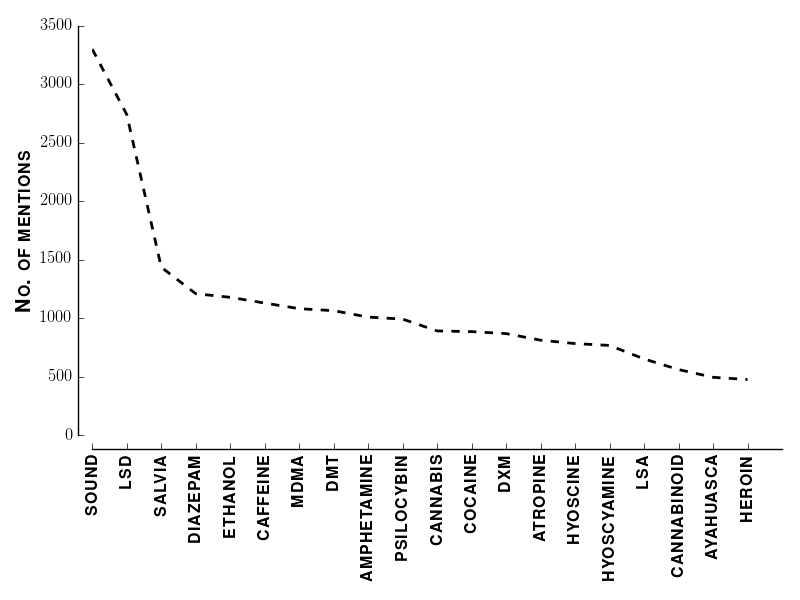
\includegraphics[scale=0.65]{overall-drug-frequency.png}
\caption{\textbf{Overall frequency of substance mentions.} $20$ most prevalent substances are shown. Refer to Table X for abbreviations.}
\label{fig:overall-f}
\end{figure}

\begin{figure}[h]
\centering
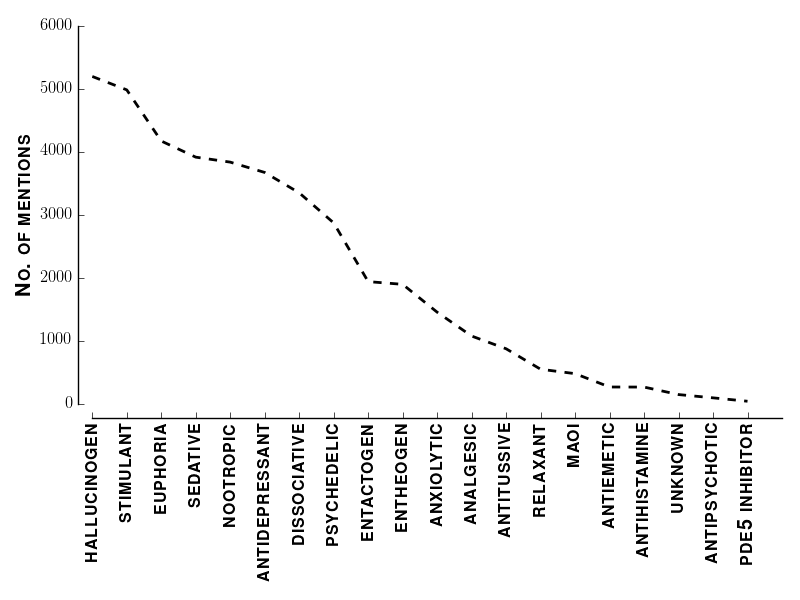
\includegraphics[scale=0.65]{effect-frequency.png}
\caption{\textbf{Overall frequency of substance effects.}}
\label{fig:effect-f}
\end{figure}

\begin{figure}[h]
\centering
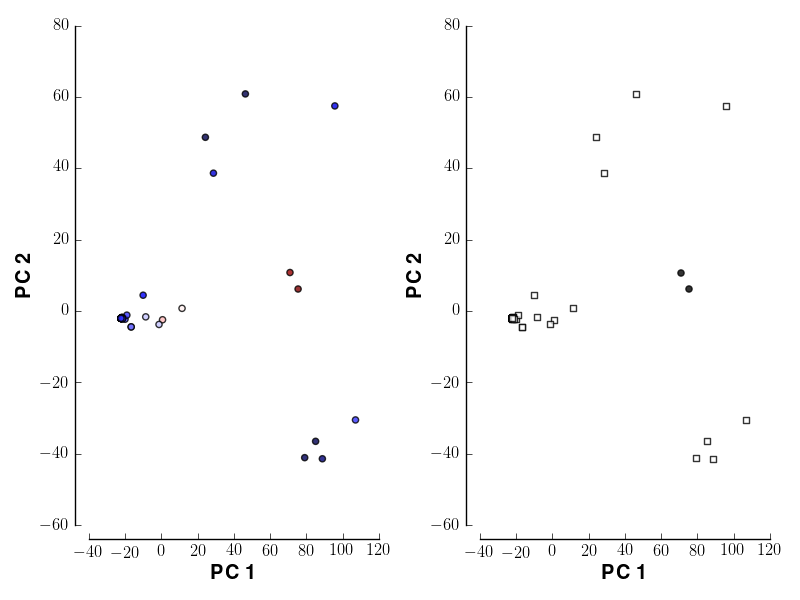
\includegraphics[scale=0.65]{effect-matrix-w-clusters.png}
\caption{\textbf{Scatter plot of drug class combinations. Left: }Projection of drug effect combinations on first two principal components. \textbf{Right:}}
\label{fig:pca}
\end{figure}

\bibliographystyle{unsrt}
\bibliography{bibliography}

\end{document}